\subsection*{Tensors}
For the purpose of this thesis we define a \textit{tensor} $T$ \textit{of rank} $n$ as an $n$-dimensional array of complex numbers
\begin{equation}
	T \in \mathbb{C}^{\chi_1\times\chi_2\times\dots\times\chi_n}, \quad \chi_i \in \{1, 2, \dots\}
\end{equation}
with entries
\begin{equation}
	T_{i_1i_2\dots i_n} \in \mathbb{C}, \quad i_j \in \{1, 2, \dots, \chi_j\}.
\end{equation}
\begin{figure}
	\centering
	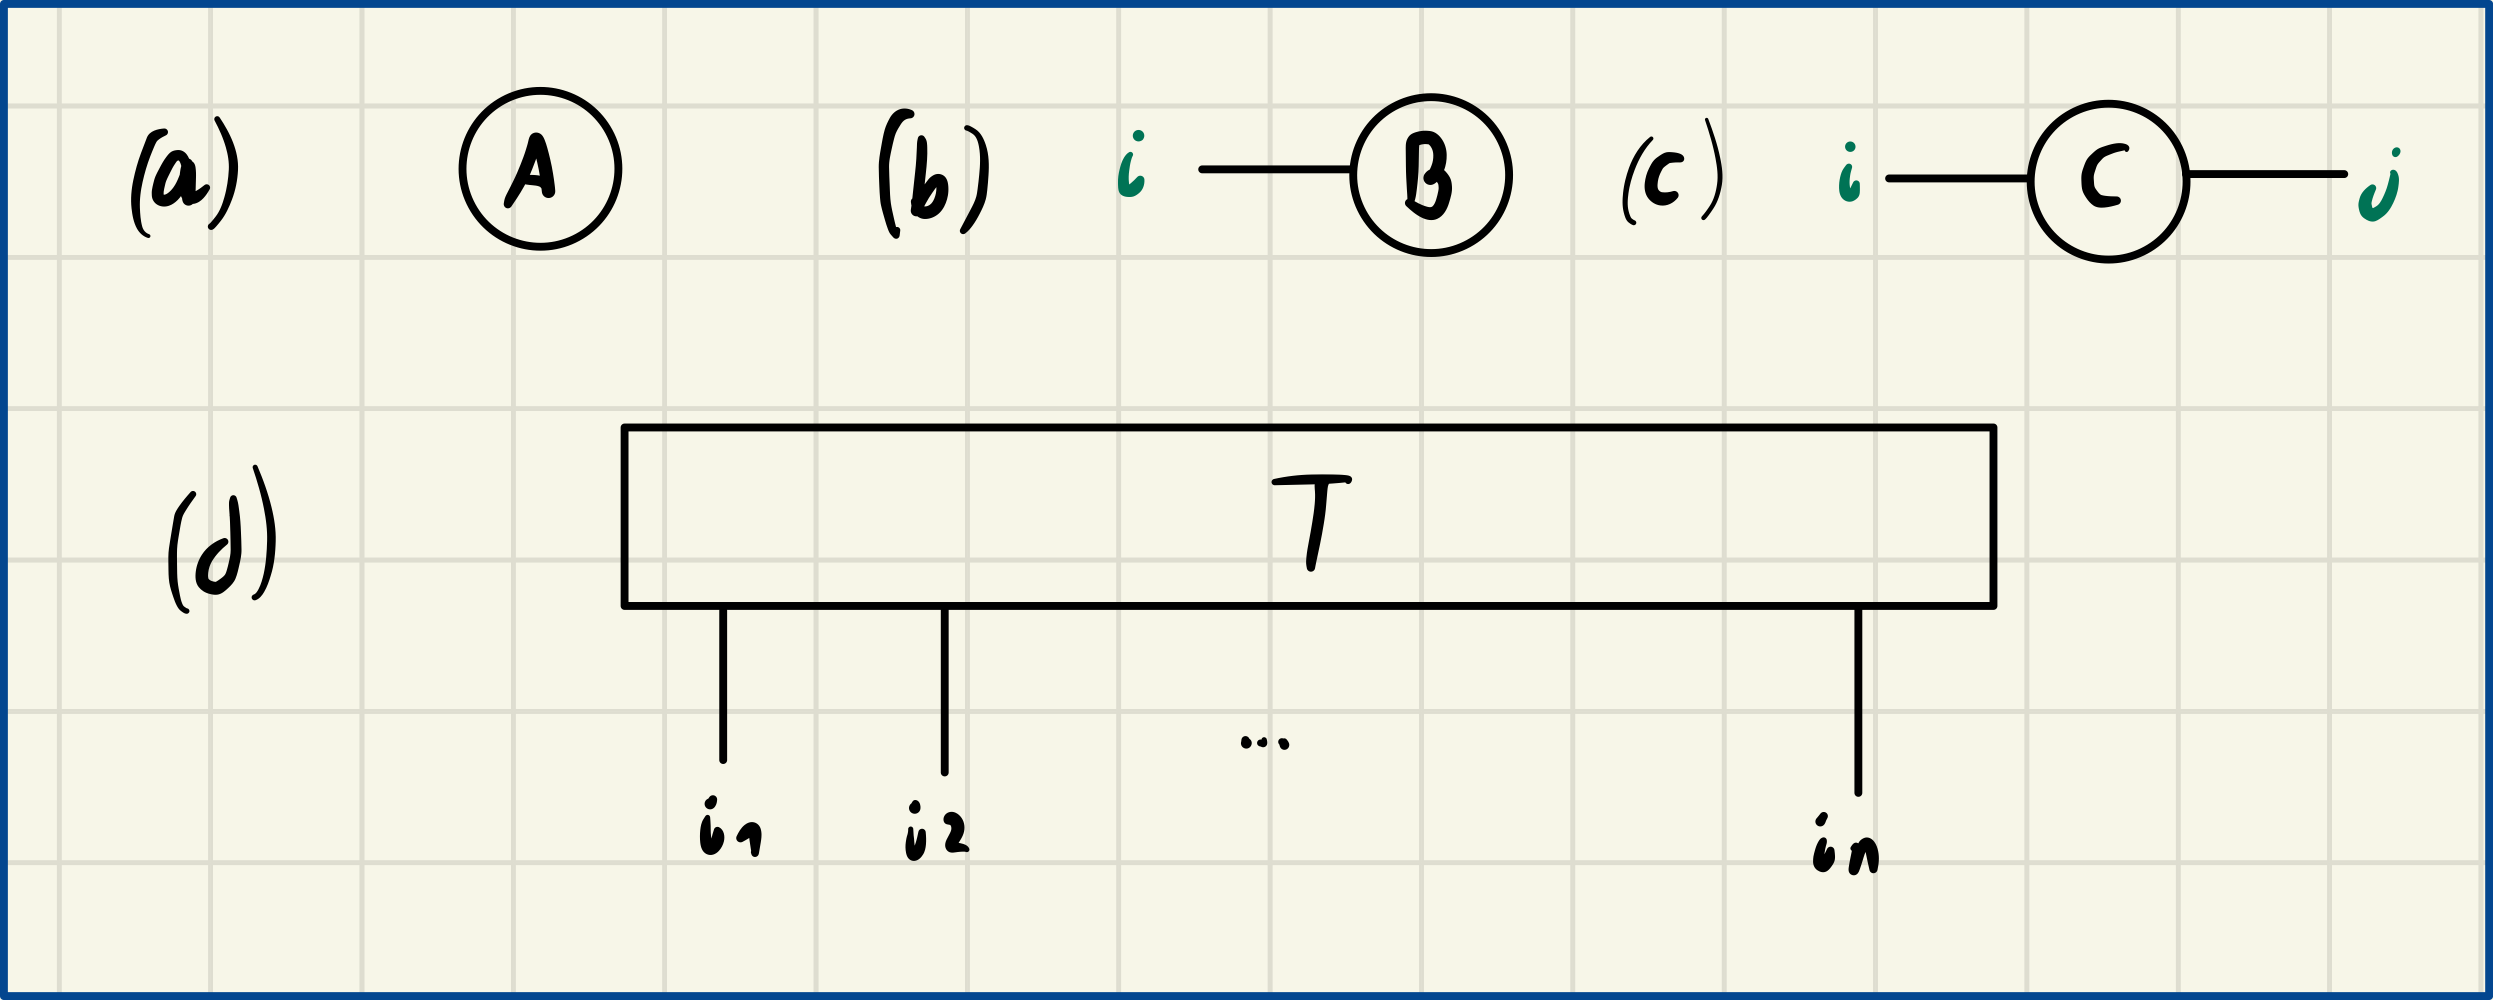
\includegraphics[width=0.8\textwidth]{figures/Tensor_Networks/basic_tensor_diagrams.jpeg}
	\caption{Tensors of different ranks are shown in diagrammatic notation.}
	\label{fig:basic_tensor_diagrams}
\end{figure}
For example, a rank-0 tensor is a scalar, a rank-1 tensor is a vector, and a tensor of rank-2 is a matrix. \par
An \textit{index contraction} between two or more tensors is the linear operation that is performed by summing over a given set of indices. For example, the matrix product of two matrices $A \in \mathbb{C}^{\chi_1\times\chi_2}$ and $B \in \mathbb{C}^{\chi_2\times\chi_3}$ can be written as the index contraction
\begin{equation}
	\label{eq:example_tensor_network_matrix_product}
	C_{ij} = \sum_{\alpha=1}^{\chi_2} A_{i\alpha} B_{\alpha j}.
\end{equation}
A more involved example is the index contraction of two rank-3 tensors $A\in\mathbb{C}^{\chi_1\times\chi_2\times\chi_3}$, $B\in\mathbb{C}^{\chi_2\times\chi_4\times\chi_5}$ and one rank-4 tensor $C\in\mathbb{C}^{\chi_3\times\chi_5\times\chi_6\times\chi_7}$, where we contract along the indices with dimension $\chi_2$, $\chi_3$ and $\chi_5$. The result is a rank-4 tensor $D\in\mathbb{C}^{\chi_1\times\chi_4\times\chi_6\times\chi_7}$:
\begin{equation}
	\label{eq:example_tensor_network_involved_network}
	D_{ijkl} = \sum_{\alpha=1}^{\chi_2} \sum_{\beta=1}^{\chi_3} \sum_{\gamma=1}^{\chi_5} A_{i \alpha \beta} B_{\alpha j\gamma} C_{\beta \gamma k l}.
\end{equation}
More generally, given a rank-$(n+f)$ tensor $A \in \mathbb{C}^{\chi_1\times\dots\times\chi_n\times\xi_{1}\times\dots\times\xi_{f}}$ and a rank-$(m+f)$ tensor $B \in \mathbb{C}^{\lambda_1\times\dots\times\lambda_m\times\xi_1\times\dots\times\xi_f}$, the result of contracting $A$ and $B$ along the last $f$ indices produces a new rank-$(m+n)$ tensor $C \in \mathbb{C}^{\chi_1\times\dots\times\chi_n\times\lambda_1\times\dots\times\lambda_m}$ as
\begin{equation}
	\label{eq:general_tensor_contraction}
	C_{i_1\dots i_nj_1\dots j_m} \coloneqq \sum_{\mu_1 = 1}^{\xi_1} \dots \sum_{\mu_f}^{\xi_f} A_{i_1\dots i_n\mu_1\dots\mu_f} B_{j_1\dots j_m\mu_1\dots\mu_f}.
\end{equation}
Contractions over arbitrary indices can be reformulated as contractions over the last $f$ indices by transposing the tensors. Contractions over more than two tensors can be decomposed into successive contractions of two tensors. Because tensor contractions are linear, the order in which tensors are contracted doesn't change the result. However, the computational complexity does in general depend on the order of contractions and can thus be minimized by choosing the optimal contraction order.\par
By counting the number of multiplications and additions that are necessary to perform the tensor contraction \eqref{eq:general_tensor_contraction}, the computational complexity can be determined as
\begin{equation}
	\label{eq:tensor_contraction_general_computational_complexity}
	\mathcal{O}\left(\prod_{\mu=1}^{n}\chi_\mu \prod_{\mu=1}^{m}\lambda_\mu \prod_{\mu=1}^{f}\xi_f\right).
\end{equation}
\subsection*{Tensor Networks}
A \textit{tensor network} is defined as a collection of tensors that are contracted in a specified way. It is convenient to introduce a diagrammatic notation, where tensors are drawn as shapes and tensor indices are represented by lines emerging from these shapes. To relate this diagrammatic notation to equations, one often decorates each line with the corresponding index $i_j$. A scalar, vector, matrix, and a general rank-$n$ tensor are visualized in this notation in figure \figref{fig:basic_tensor_diagrams}. Index contractions are depicted diagrammatically by connecting the lines corresponding to contracted indices. Lines connecting two tensors are sometimes called \textit{bonds}, while indices not used in contractions are called \textit{open indices}. The \textit{bond dimension} $\chi_i$ denotes the number of different values an index $i$ can take. It is often more convenient to discuss tensor network algorithms in terms of diagrams than in terms of equations. Two simple tensor networks are the scalar-product of two vectors
\begin{equation}
	\label{eq:example_tensor_network_scalar_product}
	c = \sum_{\alpha=1}^{\chi}A_\alpha B_\alpha
\end{equation}
and the matrix product \eqref{eq:example_tensor_network_matrix_product}. Both networks are shown as diagrams in figure \figref{fig:basic_tensor_network_diagrams}(a) and \figref{fig:basic_tensor_network_diagrams}(b) respectively. \figref{fig:basic_tensor_network_diagrams}(c) depicts the more involved tensor network \eqref{eq:example_tensor_network_involved_network}. \par
\begin{figure}
	\centering
	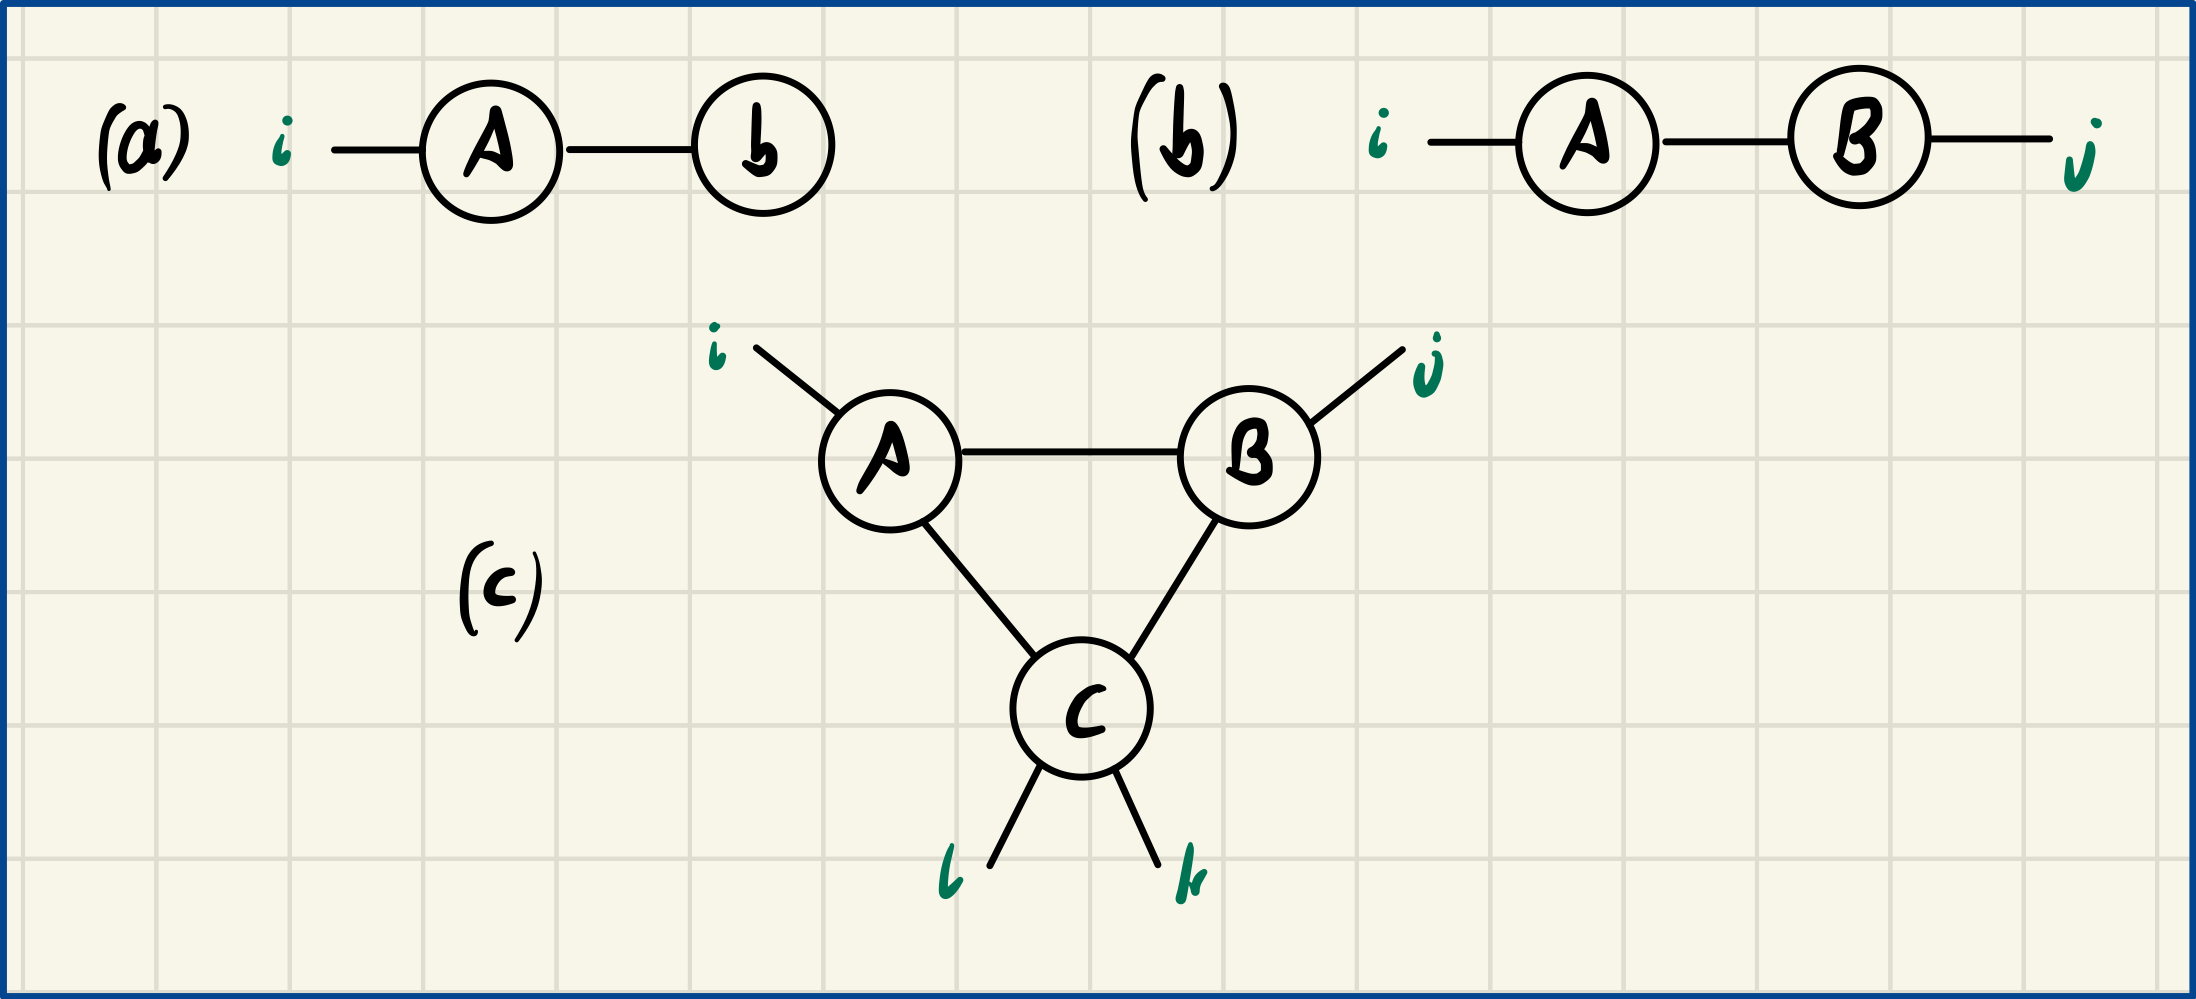
\includegraphics[width=0.8\textwidth]{figures/Tensor_Networks/basic_tensor_network_diagrams.jpeg}
	\caption{Tensor networks in diagrammatic notation. (a) Scalar product \eqref{eq:example_tensor_network_scalar_product}. (b) Matrix product \eqref{eq:example_tensor_network_matrix_product}. (c) More involved network consisting of three tensors \eqref{eq:example_tensor_network_involved_network}.}
	\label{fig:basic_tensor_network_diagrams}
\end{figure}
\subsection*{Isometries}
Given two normed vector spaces $V_1$ and $V_2$ with $\dim\left(V_1\right) = m$, $\dim\left(V_2\right) = n$, $m \le n$, an \textit{isometry} (sometimes also called \textit{semi-unitary}) is a linear, norm-preserving map $W: V_1 \rightarrow V_2$ from the smaller to the larger vector space. Each isometry can be represented by a $n\times m$ matrix $W$ fulfilling the \textit{isometry condition}
\begin{equation}
	\label{eq:isometry_condition_general}
	W^\dagger W = \id, \quad WW^\dagger = \mathbb{P},
\end{equation}
where $\mathbb{P} = \mathbb{P}^2$ is a projection. If $m = n$, it holds $\mathbb{P} = \id$ and $W$ is a \textit{unitary map}. An isometry tensor is a tensor that through grouping of indices and reshaping (i.e. matricization) becomes an isometry. In tensor network diagrams, we draw isometries by decorating lines with arrows. Following the convention of \cite{cite:isometric_tensor_network_states_in_two_dimensions, cite:efficient_simulation_of_dynamics_in_two_dimensional_quantum_spin_systems}, we denote the indices belonging to the larger vector space by incoming arrows and the indices belonging to the smaller vector space by outgoing arrows. Unitary tensors are decorated with bidirectional arrows on all indices, where the grouping must be inferred from the context. Ordinary tensors are drawn without arrows. Tensor diagrams for isometric and unitary tensors are shown in figure \figref{fig:isometries_and_unitaries_diagrams}.\par
\begin{figure}
	\centering
	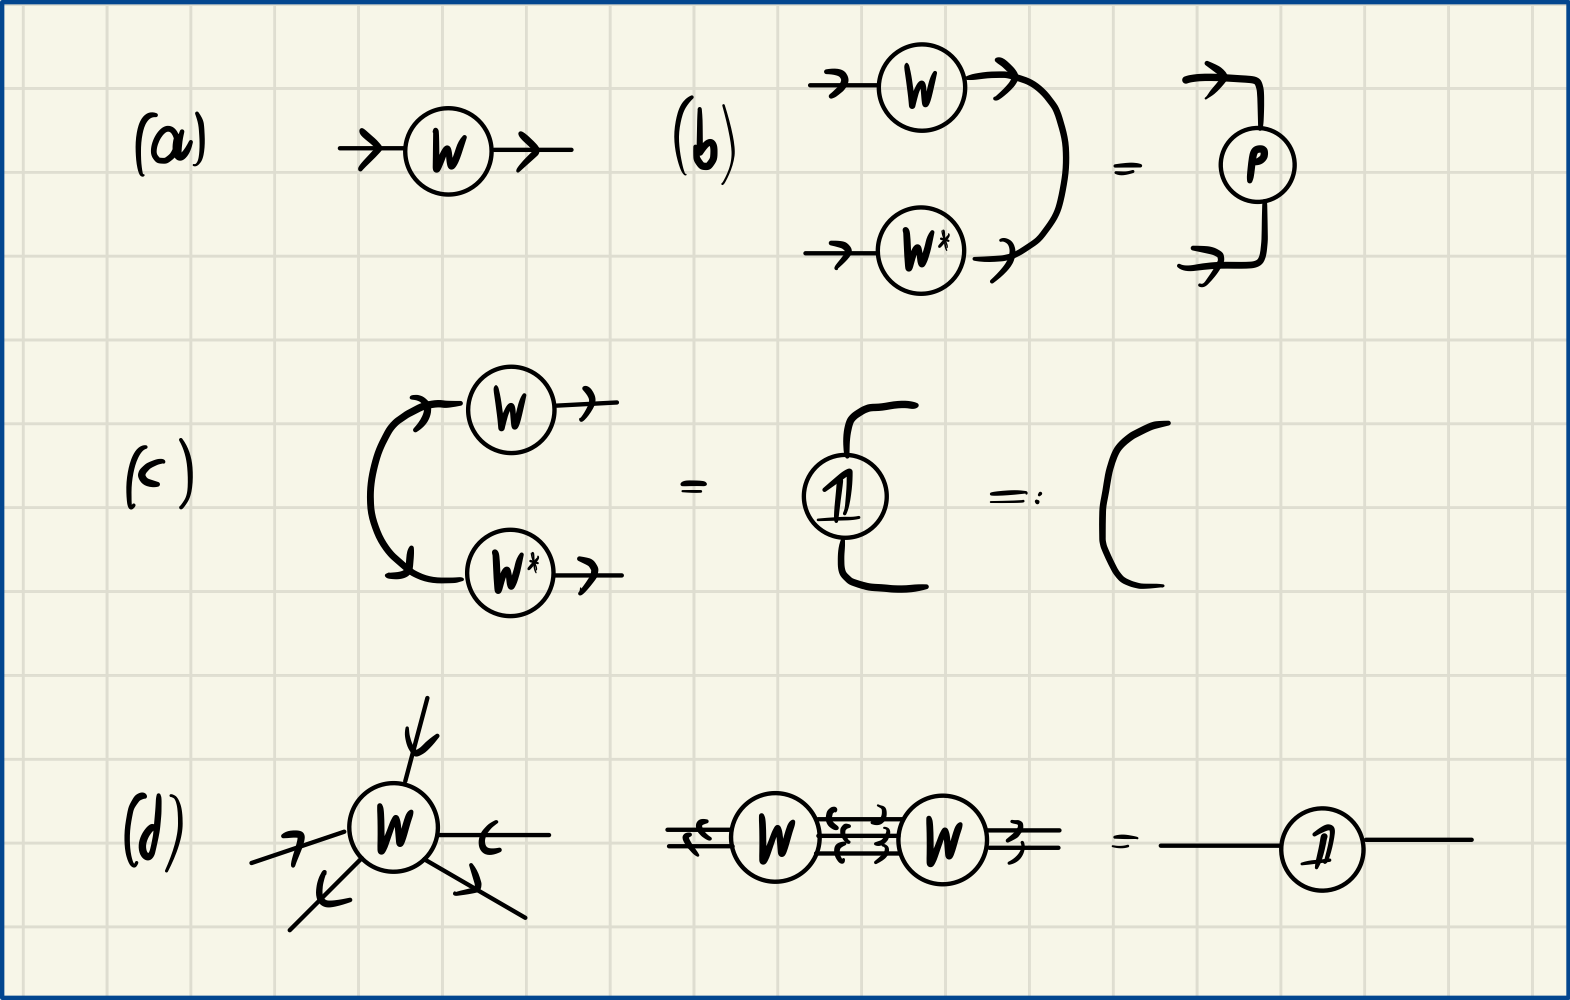
\includegraphics[width=0.8\textwidth]{figures/Tensor_Networks/basic_isometric_tensor_diagrams.jpeg}
	\caption{Isometric and unitary tensors are drawn by decorating indices with arrows. (a) diagrammatic notation of an isometric matrix (b) (c) The isometry condition \eqref{eq:isometry_condition_general} is depicted diagrammatically. (d) Isometric tensors of higher rank must fulfill the isometry condition by grouping of indices.\todo{Add unitary tensor as well with double arrows}}
	\label{fig:isometries_and_unitaries_diagrams}
\end{figure}
We lastly introduce an inner product for rank-$n$ tensors $A, B \in \mathbb{C}^{\chi_1\times\dots\times\chi_n}$, the \textit{Frobenius inner product}
\begin{equation}
	\label{eq:frobenius_inner_product}
	\left\langle A, B\right\rangle_\text{F} \coloneqq \sum_{\mu_1=1}^{\chi_1} \dots \sum_{\mu_n=1}^{\chi_n} A_{\mu_1\dots\mu_n}^*B_{\mu_1\dots\mu_n} = \Tr\left(A^\dagger B\right),
\end{equation}
where the last equality holds only if $n = 2$. The Frobenius inner product induces a norm, the \textit{Frobenius norm}
\begin{equation}
	\label{eq:frobenius_norm}
	\lVert A\rVert_\text{F} = \sqrt{\left\langle A, A\right\rangle_\text{F}},
\end{equation}
which can be used to define a measure of distance $\lVert A-B\rVert_\text{F}$ between tensors $A$ and $B$.